\jeff{Bruce wants us to write a paragraph about the importance of GPUs for MD calculations. I really don't have any experience with MD, so I have no idea what to write here. Does anyone else have something interesting to say?}

A major performance bottleneck of \osprey designs with continuous flexibility is minimizing protein conformations and conformation fragments. Since the space of possible conformations in a design grows exponentially with the number of flexible and mutable residues, the number of conformations that must (in the worst-case) be enumerated to find the GMEC or to approximate the Boltzmann-weighted partition function grows exponentially as well. Since all enumerated conformations must be subsequently minimized to compute their energies, and minimization is a relatively expensive operation, the bulk of a design's runtime can be spent on energy minimization of conformations. Therefore, improvements to the speed of energy minimization (an operation that is called an exponential number of times) can have a dramatic impact on \osprey runtimes.

Much work has been done in the past to optimize \osprey for execution on CPUs, particularly highly multi-core CPUs and even networked clusters of CPU-powered servers~\cite{minBounds_DACS,cloud_OSPREY}. However, modern GPU hardware enables high-performance computation at a fraction of the cost of large CPU clusters, mainly due to the huge video game industry that propels innovation in hardware design and drives down costs. \osprey3 includes GPU programs (called {\it kernels}) built using the CUDA framework~\cite{nvidia2010programming} that implements the forcefield calculations and local minimization algorithms used in protein redesign.

We present performance results of these GPU kernels on various hardware platforms in Figure~\ref{fig:gpu}. A GPU server housing 4 Nvidia Tesla P100 cards can finish minimizations with about 300,000 atom pairs roughly 110-fold faster than a single thread running on an Intel Xeon E5-2640 v4 CPU. With two Intel Xeon E5-2640 v4 CPUs running at full capacity with multiple threads, the four Nvidia Tesla P100 GPUs finish the same minimizations roughly 8-fold faster. The speedups of GPUs over CPUs scale with the number of atom pairs in the minimization. For minimizations with fewer atom pairs, even four Nvidia Tesla P100 GPUs cannot outperform two Intel Xeon E5-2640 v4 CPUs. There is significant overhead to transfer each minimization problem from the CPU to the GPU during designs. Even though GPUs can evaluate the minimizations much faster than CPUs, when there are few atom pairs, this transfer overhead dominates the computation time and causes GPUs to perform merely similarly to CPUs, rather than significantly faster.

The performance of desktop hardware appears similar to server hardware, except on a smaller scale. A single Nvidia GTX 1070 GPU performs minimizations at roughly half the speed of an Nvidia Tesla P100 GPU. Two Nvidia GTX 1080 GPUs perform similarly to the Nvidia Tesla P100 GPU on the large conformation benchmark, but actually perform worse than a single Nvidia GTX 1070 for the small conformation benchmark -- despite having well over twice the hardware of the single Nvidia GTX 1070 GPU. This anomalous performance suggests the kernel \osprey3 uses for minimizations is not yet well-optimized for the Nvidia GTX 1080 GPU, and that future engineering efforts could offer significant performance increases for Nvidia GTX 1080 GPUs. The Nvidia GTX 1050, a laptop GPU, does not appear to be powerful enough to offer any advantages over traditional CPU computing in \osprey3.

Modern GPU architectures offer thousands of parallel hardware units for calculations, compared to the tens of parallel hardware units in modern CPU architectures. The performance results of the current generation of \osprey's GPU kernels indicate that minimization speeds on GPUs have only begun to scratch the surface of what is possible, particularly for minimizations with few atom pairs. Future versions of these GPU kernels will likely offer significantly higher performance on the same hardware -- perhaps allowing minimization speeds many times faster than today's GPU kernels.

\begin{figure}
\center
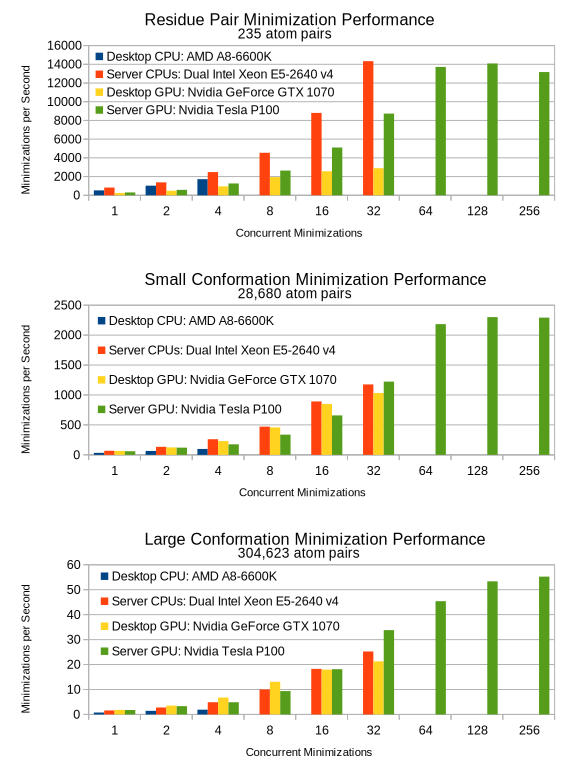
\includegraphics[width=4in]{figures/gpu.pdf}
\caption{Benchmarks for protein conformation minimization in \osprey3 for various hardware platforms and for conformations of varying size. From smallest to largest: {\bf (top)} a single residue pair is the smallest multi-body minimization possible, {\bf (middle)} a full protein conformation with a single flexible residue represents a small design, {\bf (bottom)} a full protein conformation with 20 flexible residues represents a large design. For CPU hardware, concurrent minimizations correspond to CPU threads. For GPU hardware, concurrent minimizations correspond to {\it streams} defined by the CUDA framework. Faster minimization speeds correspond with faster \osprey runtimes. All minimizations were performed on the Atx1 metallochaperone protein (PDB ID: 1CC8)~\cite{1CC8}. Flexible residues were modeled with continuous sidechain flexibiltiy, and all other residues remained completely fixed.}
\label{fig:gpu}
\end{figure}
